\section{Requirements Specification}

\subsection{Overview}
\frame{
\frametitle{Intention}
\begin{figure}[!htb]
\begin{center}
\resizebox{.60\textwidth}{!}{\includegraphics{figures/main.ps}}
\end{center}
\end{figure}
}
\subsection{g: VDM++ $\rightarrow$ JML}
\frame{
\frametitle{Parsing and AST generation}
\begin{figure}[!htb]
\begin{center}
\resizebox{.99\textwidth}{!}{\includegraphics{figures/vdmParser.ps}}
\end{center}
\end{figure}
}
\frame{
\frametitle{Converting ASTs and generating JML code}
\begin{figure}[!htb]
\begin{center}
\resizebox{.99\textwidth}{!}{\includegraphics{figures/vdmConvertAsts.ps}}
\end{center}
\end{figure}
}
\subsection{f: JML $\rightarrow$ VDM++}
\frame{
\frametitle{Parsing JML files and AST generation}
\begin{figure}[!htb]
\begin{center}
\resizebox{.86\textwidth}{!}{\includegraphics{figures/diagramaChecker.ps}}
\end{center}
\end{figure}
}
\frame{
\frametitle{AST conversion}
\begin{figure}[!htb]
\begin{center}
\resizebox{.99\textwidth}{!}{\includegraphics{figures/diagramaConvertASTs.ps}}
\end{center}
\end{figure}
}
\frame{
\frametitle{VDM++ code generation}
\begin{figure}[!htb]
\begin{center}
\resizebox{.99\textwidth}{!}{\includegraphics{figures/diagramaJMLVDM.ps}}
\end{center}
\end{figure}
}
\subsection{Tool support to use}
\frame{
\frametitle{Tool support}
VDM++/Overture tool support:
\newline
\pause
\begin{itemize}
\item Overture parser
\pause
\item Overture AST generator
\pause
\item VDMTools Java Code Generator
\pause
\end{itemize}
JML tool support:
\newline
\pause
\begin{itemize}
\item JML Checker
\end{itemize}
}

\subsection{Tool support to develop}
\frame{
\frametitle{Tool support}
\begin{itemize}
\item JML abstract syntax tree
\pause
\item JmlAst to JmlAstVdm mapper
\pause
\item JmlAstVdm to Vdm++Ast mapper
\pause
\item Vdm++Ast to JmlAstVdm mapper
\pause
\item pretty printer(s)...
\end{itemize}
}